\documentclass[tikz]{standalone}
\begin{document}
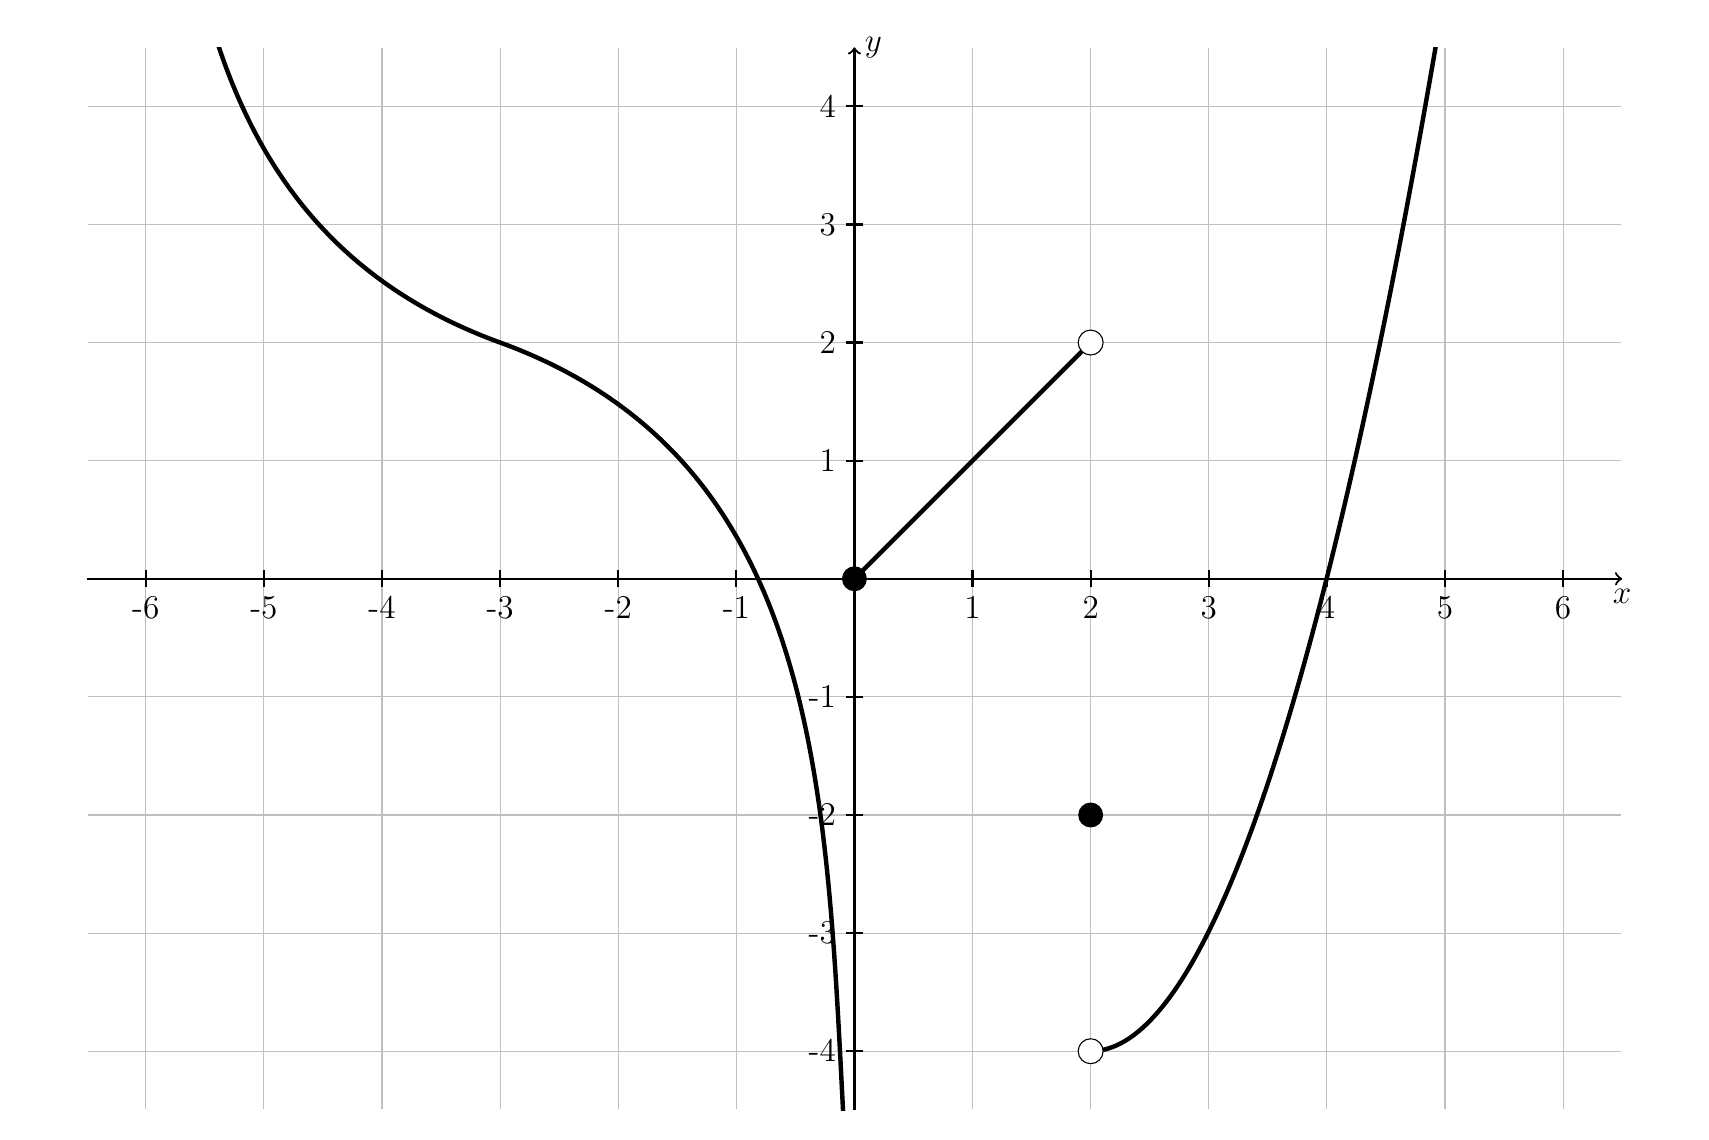
\begin{tikzpicture}[scale=1.5]
\tikzstyle{every node}=[font=\large]

% create a white background, with a black frame
%\draw [fill=white,white] (-7,-5) rectangle (7,5); 

% draw a grid
\draw[step=10mm, lightgray, thin] (-6.49,-4.49) grid (6.49,4.49); 
%\draw[step=1cm, gray] (0,-0) grid (6.5,3.5); 

% draw axes
\draw [->,thick] (-6.5,0) -- (6.5,0) node[below] {$x$}; 
\draw [->,thick] (0,-4.5) -- (0,4.5) node[right] {$y$};

% tick marks
\foreach \x in {-6,-5,...,-1,1,2,...,6} 
	\draw [thick] (\x cm,2pt) -- (\x cm,-2pt) node[below] {\x};
\foreach \y in {-4,-3,...,-1,1,2,...,4} 
	\draw [thick] (2pt,\y cm) -- (-2pt,\y cm) node[left] {\y};

% plot curve
\clip (-7,-4.5) rectangle (7,4.5);
\draw [ultra thick] (-6,10) to [out=-85,in=160] (-3,2) to [out=-20,in=95] (0,-6);
\draw [ultra thick] (0,0) -- (2,2);
\draw [ultra thick] (2,-4) parabola (6,12);

% \plot points
\fill (0,0) circle (3pt);
\draw [fill=white] (2,2) circle (3pt);
\fill (2,-2) circle (3pt);
\draw [fill=white] (2,-4) circle (3pt);

\end{tikzpicture}
\end{document}
